\documentclass{beamer}

\mode<presentation>
{
  \usetheme{CambridgeUS}
  \setbeamercovered{transparent}
}

\usepackage{amsmath}
\usepackage[english]{babel}
\usepackage[latin1]{inputenc}
\usepackage{times}
\usepackage[T1]{fontenc} 

% The text in square brackets is the short version of your title and will be used in the
% header/footer depending on your theme.
\title[Zero Knowledge Compilers]{Zero Knowledge Compilers}

% Sub-titles are optional - uncomment and edit the next line if you want one.
% \subtitle{Why does sub-tree crossover work?}

% The text in square brackets is the short version of your name(s) and will be used in the
% header/footer depending on your theme.
\author[McCall]{John McCall}
\institute[U of Minn, Morris]
{
  Division of Science and Mathematics \\
  University of Minnesota, Morris \\
  Morris, Minnesota, USA
}

\AtBeginSection[]
{
  \begin{frame}<beamer>
    \frametitle{Outline}
    \tableofcontents[currentsection, hideothersubsections]
  \end{frame}
}

\begin{document}

\begin{frame}
	\titlepage
\end{frame}

\section*{Overview}

\begin{frame}
	\frametitle{Overview}
	\begin{itemize}
		\item Zero knowledge protocols are used to prove the validity of a statement, without revealing anything other than the correctness of the claim.
		\item They have practical applications in cryptography.
		% Such as Direct Anonymous Attestation.
		
		\item They are difficult to design and to implement.
		
		\item Zero knowledge compilers help to ease this burden.
	\end{itemize}
\end{frame}

\begin{frame}
	\frametitle{Outline}
	\tableofcontents[hideallsubsections]
\end{frame}

\section{Zero Knowledge Protocols}

\begin{frame}
	\frametitle{Zero Knowledge Proofs}
	\begin{itemize}
		\item Consist of a prover and a verifier.
		
		\item Can be used to prove knowledge of a statement.
		
		\item Are a type of interactive proof.
	\end{itemize}
\end{frame}

\begin{frame}
	\frametitle{Interactive Proof}
	Must satisfy:
	\begin{itemize}
		\item \textit{Completeness:} If the statement being proven is true, an
		honest verifier, a verifier correctly following the protocol, will be
		convinced after interacting with an honest prover.

		\item \textit{Soundness:} If the statement is false, no prover, either
		honest or dishonest, will be able to convince an honest verifier, except
		with some small probability.
	\end{itemize}
\end{frame}

\begin{frame}
	\frametitle{Zero Knowledge Proof}
	Must satisfy:
	\begin{itemize}
		\item \textit{Zero knowledge:} Any knowledge known by
	the prover or the verifier before performing the proof is the same
	as the knowledge known by either party after performing the proof.		
	\end{itemize}
\end{frame}

\subsection{Magic Cave}

\begin{frame}
	\frametitle{Setup}
	\begin{figure}
	\centering
	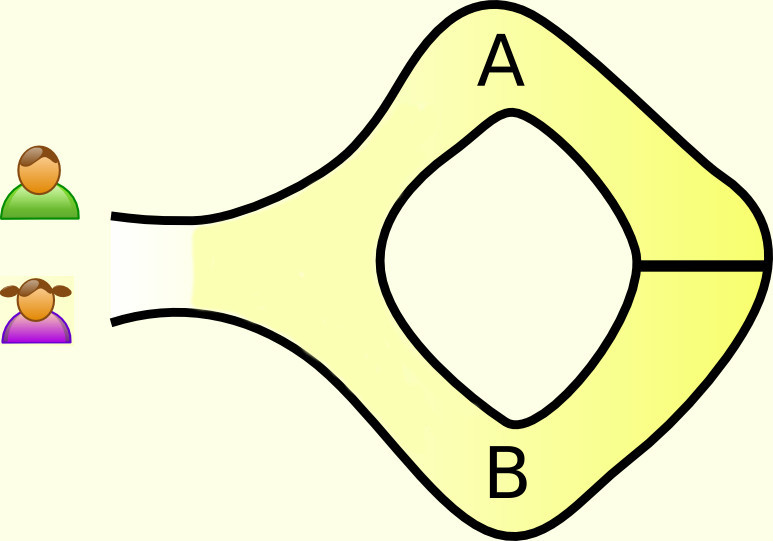
\includegraphics[width=0.70\textwidth]{MagicCave0.jpg}
	\caption{An image of the cave. \linebreak Modified from: \url{wikipedia.org/wiki/Zero-knowledge_proof}}
	\label{fig:MCave}
	\end{figure}
	
\end{frame}

\begin{frame}
	\frametitle{Protocol}

	\begin{figure}
	\centering
	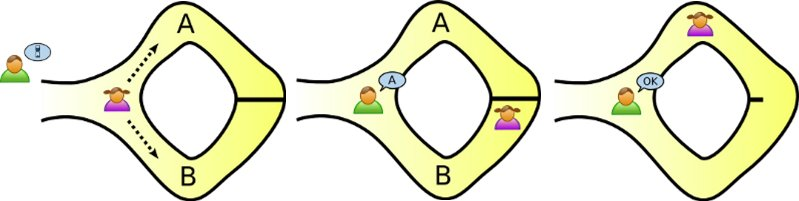
\includegraphics[width=1.00\textwidth]{MagicCave.jpg}
	\caption{Illustration of the magic cave protocol. \linebreak Taken from: \url{wikipedia.org/wiki/Zero-knowledge_proof}}
	\label{fig:MCave}
	\end{figure}
	
\end{frame}

\subsection{Hamiltonian Cycles}

\begin{frame}
	\frametitle{Definitions}
	\begin{itemize}
		\item A \textit{cycle} is a list of connected vertices of a graph
		which starts and ends at the same vertex. 
		
		\item A \textit{Hamiltonian path} is a list of connected vertices of a
		graph which includes each vertex exactly once.
		
		% I probably want a picture of a Hamiltonian Cycle
		\item A \textit{Hamiltonian cycle} is a Hamiltonian path which is also
		a cycle.
		
	\begin{figure}
	\centering
	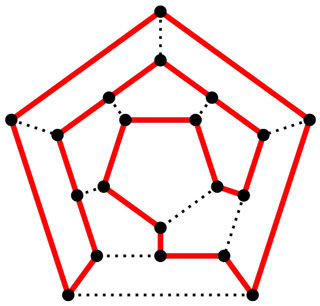
\includegraphics[width=0.30\textwidth]{HCycle.jpg}
	\caption{An example of a Hamiltonian cycle. The solid line marks the path.
	Taken from: \url{wikipedia.org/wiki/Hamiltonian_path}}
	\label{fig:HCycle}
	\end{figure}
		
		% Talk about how finding a Hamiltonian Cycle is NP-Complete.
	\end{itemize}
\end{frame}

\begin{frame}
	\frametitle{Definitions}
	\begin{itemize}
		\item An \textit{isomorphism}, $f: V(G) \rightarrow V(H)$, of graphs 
		$G$ and $H$ is a 
		bijection between the vertex
		sets of $G$ and $H$ such that any two vertices $u$ and $v$ are
		adjacent in $G$ if and only if $f(u)$ and $f(v)$ are adjacent in $H$.
	\end{itemize}
\end{frame}

\begin{frame}
	\frametitle{One-way Functions}
	\begin{itemize}
		
		\item Difficult to reverse.
		
		\item Low probability of collisions.
		
		\item Used when the prover needs to choose a value which remains a secret at first, but will be revealed later.
		
	\end{itemize}
\end{frame}

\begin{frame}
	\frametitle{Setup}
	\begin{itemize}
		\item Want to prove knowledge of a Hamiltonian cycle in a graph without
		revealing the cycle.
		
		\item Peggy knows a Hamiltonian Cycle for a graph, $G$.
		Victor has knowledge of $G$ but not the cycle.
	\end{itemize}
\end{frame}

\begin{frame}
	\frametitle{Protocol}
	\begin{itemize}
		\item Peggy constructs $H$, a graph which
		is isomorphic to $G$. Since Peggy knows a Hamiltonian cycle
		for $G$ she must know one for $H$ as well.
		
		\item Peggy commits to $H$, using a one-way function. Doing this 
		means that Peggy cannot change $H$ without Victor finding	out.
		
		\item Victor then randomly asks Peggy to do one of two things. Either show
		the isomorphism between $H$ and $G$, or show a Hamiltonian cycle in $H$.		
	\end{itemize}
\end{frame}

\begin{frame}
	\frametitle{Protocol}
	\begin{itemize}
		\item If Peggy was asked to show that the two graphs are isomorphic, she
		starts by revealing $H$ to Victor. She also reveals the isomorphism between 
		$G$ and $H$. Victor can then verify that the two graphs are isomorphic.
		
		\item If Peggy was asked to show a Hamiltonian cycle in $H$, she first 
		translates the cycle from $G$ onto $H$. She then reveals to Victor the 
		Hamiltonian cycle in $H$. 
		
		\item In both cases Victor must also verify that $H$ is the same graph 
		that Peggy committed to by using the same one-way function and comparing 
		the outputs.
		
		%Explain how Peggy can cheat.
		
	\end{itemize}
\end{frame}

\section{Compilers}

\begin{frame}
	\frametitle{Compilers}
	\begin{itemize}
		\item Translates one language into another. 
		\item Many different types of compilers: single-pass compilers, multi-pass, optimizing compilers, and many others.
		\item The first compilers started to appear in the 1950s.
		\item Notoriously difficult to implement, at the time.
		\item There are two parts to compilation, analysis and synthesis.
	\end{itemize}
\end{frame}

\begin{frame}
	\frametitle{Zero Knowledge Compilers}
	\begin{itemize}
		\item Take, as input, an abstract proof specification or proof-goal, 
		written in languages designed specifically for this problem.
		%Mention that the languages are supposed to reflect a proof goal
		\item Output an implementation of the given specification in
    a high-level language, usually C++ or Java.
	\end{itemize}
\end{frame}

\section{Zero Knowledge Compilers}

\subsection{Background}

\begin{frame}
	\frametitle{Definitions}
	
	 A \textit{group}, in a mathematical sense, is a set, $G$ paired with an 
		operation, $\odot$. Written as $(G, \odot)$
		
		\begin{itemize}
			\item The set must be closed under that operation.
				\begin{itemize} 
					\item If $a, b \in G$ then $a \odot b \in G$.
				\end{itemize}
			\item The operation must be associative.
				\begin{itemize} 
					\item If $a, b, c\in G$ then $(a \odot b) \odot c = a \odot (b \odot c)$.
				\end{itemize}
			\item There must be an identity element.
				\begin{itemize} 
					\item There exists an $e \in G$ such that for all $a \in G, a \odot e = a$.
				\end{itemize}
			\item There must be	an inverse element.
				\begin{itemize} 
					\item For all $a \in G$, there exists an $a^{-1} \in G$ such that, $a \odot a^{-1} = e$.
				\end{itemize}
		\end{itemize}
\end{frame}

\begin{frame}
	\frametitle{Definitions}
	\begin{itemize}
		\item The \textit{preimage} of a set, $B$, under some function,
		$f:A \rightarrow B$, is the set of all elements $a$ in $A$ such
		that $f(a)$ is in $B$.
		
		\item For example, if $f(x) = x^{2}$ then the preimage of $\{4\}$
		would be $\{-2, 2\}$
	\end{itemize}
	
	%add a diagram 
\end{frame}



\begin{frame}
	\frametitle{Definitions}
	\begin{itemize}
		\item A mapping $\phi : G \rightarrow H$ from a group, $(G, \odot)$, 
		to another group,  $(H, \oplus)$, is called a \textit{homomorphism} 
		if and only if for all $a, b$ in $G$ the following equation holds:
		$\phi(a \odot b) = \phi(a) \oplus \phi(b)$
	\end{itemize}
\end{frame}

\begin{frame}
	\frametitle{Homomorphism}
	
	\begin{figure}
	\centering
	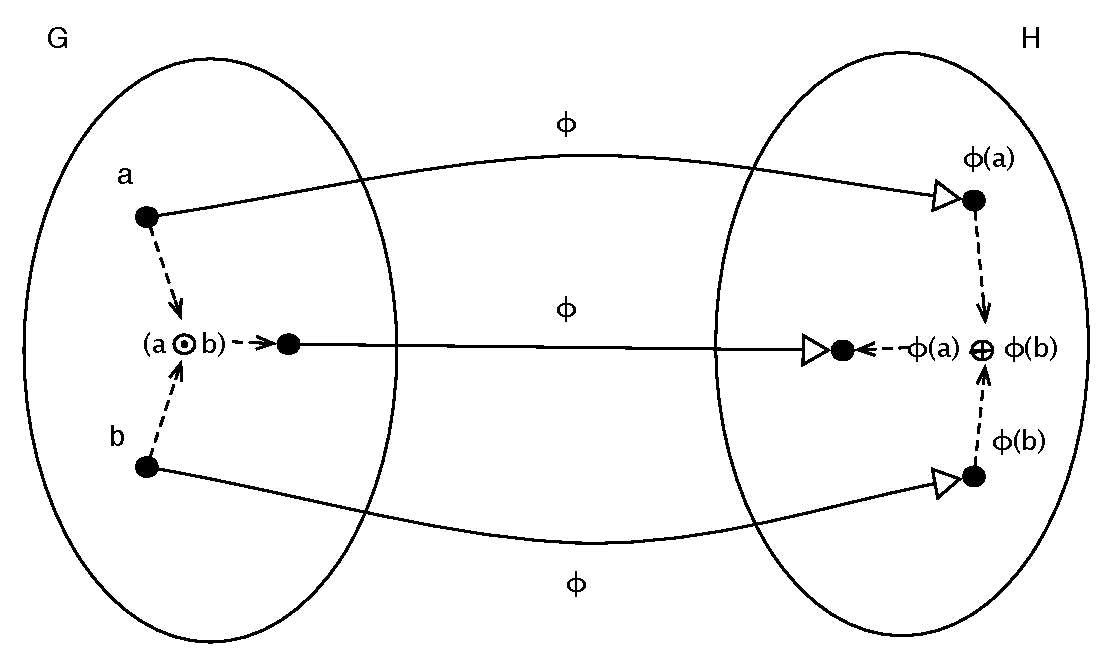
\includegraphics[width=0.80\textwidth]{homomorphism.pdf}
	\caption{Diagram showing a homomorphism.}
	\label{fig:HCycle}
	\end{figure}
\end{frame}

\subsection{ZKCrypt}

\begin{frame}
	\frametitle{ZKCrypt}
	\begin{itemize}
		\item Developed by Almedia et al.
		\item An optimizing cryptographic compiler.
		%\item Based on $\Sigma$-protocols.
		\item Utilizes \textit{verified compilation} and \textit{verifying compilation}.
	\end{itemize}
\end{frame}

\begin{frame}
	\frametitle{ZKCrypt}
	
	\begin{figure}
	\centering
	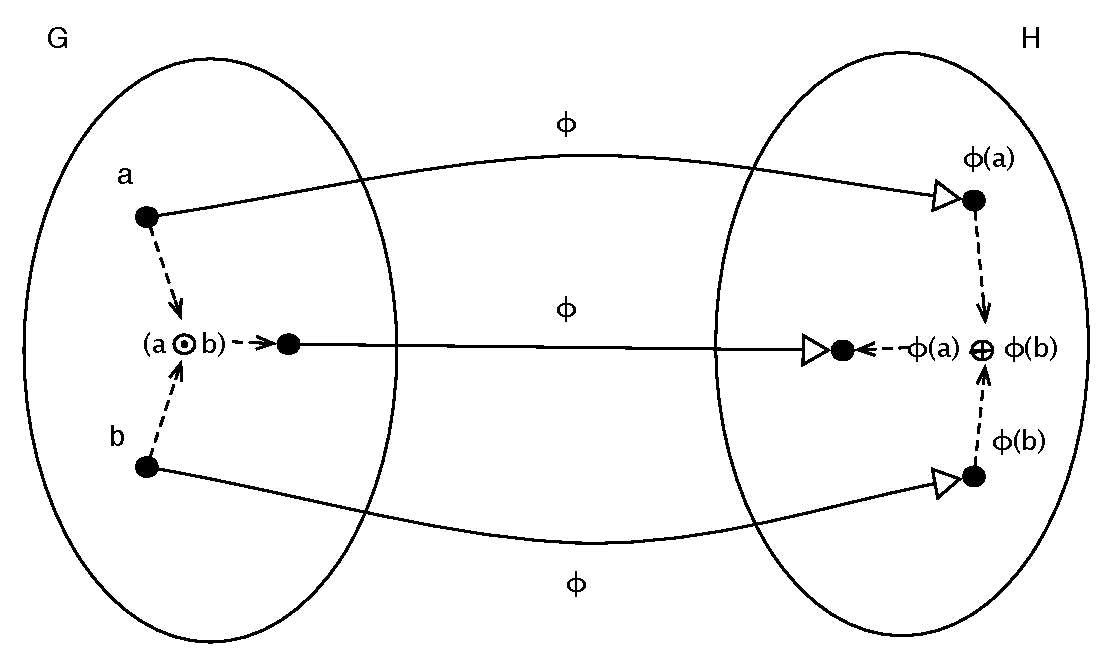
\includegraphics[width=0.80\textwidth]{homomorphism.pdf}
	\caption{Diagram showing a homomorphism.}
	\label{fig:HCycle}
	\end{figure}
\end{frame}

\begin{frame}
	\frametitle{The Input}
	Consists of:
	\begin{itemize}
		\item Declarations block.
		
		\item Inputs block.
		
		\item Protocol block:
		\begin{itemize}
			\item Homomorphism.
			\item Relation.
		\end{itemize}
	\end{itemize}
\end{frame}

\begin{frame}
	\frametitle{ZKCrypt}
	\begin{itemize}
		\item \textit{Verified compilation} is where the correctness of the output is proven once-and-for-all.
		\item \textit{Verifying compilation} is where the correctness of the output is checked on each run.
	\end{itemize}
\end{frame}

\subsection{ZKPDL}

\begin{frame}
	\frametitle{ZKPDL}
	\begin{itemize}
		\item Developed by Meiklejohn et al.
		
		\item Primarily used in electronic cash.
		
		\item Split into independent two blocks: \textit{computation} and \textit{proof}.
		
	\end{itemize}
\end{frame}

\begin{frame}
	\frametitle{The Input}
	\begin{itemize}
		\item Computation block:
		\begin{itemize}
			\item Given block.
		
			\item Compute block.
		
		\end{itemize}
	
		\item Proof block:
		\begin{itemize}
			\item Given block.
		
			\item Prove knowledge of block.
		
			\item Such that block.
		\end{itemize}
	\end{itemize}
\end{frame}

\section{Conclusion}

\begin{frame}
	\frametitle{Final Thoughts}
	\begin{itemize}
		\item ZKCrypt, more general purpose, performs optimizations.
		
		\item ZKPDL, more focused on e-cash.
				
	\end{itemize}
\end{frame}

\section*{References}

\begin{frame} 
        \frametitle{References} 
        
        \begin{thebibliography}{lskdjf}
        
        \bibitem{ZKCrypt}
J.~B. Almeida, M.~Barbosa, E.~Bangerter, G.~Barthe, S.~Krenn, and S.~Z. B{\'e}guelin.
\newblock Full proof cryptography: verifiable compilation of efficient zero-knowledge protocols.
\newblock In \textit{Proceedings of the 2012 ACM conference on Computer and communications security}, {\em CCS '12}, pages 488-500, ACM, New~York, New~York, USA, 2012.
        
        \bibitem{citeulike:3452411}
        S.~Meiklejohn, C.~Erway, A.~K\"{u}p\c{c}\"{u}, T.~Hinkle,and A.~Lysyanskaya.
\newblock ZKPDL: a language-based system for efficient zero-knowledge proofs and electronic cash.
\newblock In Proceedings of the 19th USENIX conference on Security , {\em USENIX Security'10}, USENIX Association, Berkeley, CA, USA.
  
          \end{thebibliography}

\end{frame}

\section*{Questions?}

\begin{frame}
	\frametitle{Thank you!}
	\Large{Questions?}
\end{frame}





\end{document}